\section{Results and Discussion} \label{results}



\subsection{Performance}\label{performance}
The temporal dynamics of a molecular system can be described by the \acrfull{cme}\cite{kampen_stochastic_2011}.
\acrfull{ssa}\cite{gillespie_general_1976} simulates these stochastic dynamics directly returning a set of individual trajectories for a list of particles observed.
In order to obtain accurate estimates of the average dynamic within a population of cell (\ie{} the mean dynamics), it is however necessary to perform multiple (often more than $10^4$) simulations.
Despite recent efforts \cite{niemi_efficient_2011,dittamo_optimized_2009,komarov_accelerating_2012} to provide fast implementation of this algorithm, computation remains extremely expensive. 
This time-complexity is a limiting factor in downstream analysis techniques, for
instance parameter inference that often requires repetition of these experiments for a large set of parameter values.

This particular limitation led to the development of approximations such as \acrfull{lna}\cite{komorowski_bayesian_2009} and \acrfull{mea}\cite{ale_general_2013}
 which model the mean behaviour directly, without evaluating the individual particle behaviours, and therefore can perform in a more realistic time.

Since the main driving force for development of these approximation algorithms is the potential reduction of the time taken to perform the analysis, 
it is paramount to make the implementation as efficient as possible.

In this section, we explore the implementation factors that influence the runtime of the algorithm, and describe the optimisations done to increase the its performance.
In particular, we show that symbolic computations can be limiting the algorithm and explain the techniques used to optimised them.
We also quantify the increase in performance we achieved and show that it is several orders of magnitude faster than the original \mat{} prototype.
In addition, we explore other limiting factors we have less control of, such as the choice of \gls{ode} solver, and discuss their potential implications to the analysis of biological systems.

\subsubsection{Optimising \acrlong{mea}}
\label{sec:optimising_mea}

\gls{mea} involves derivation of a system \gls{ode}s from a model.
This procedure\cite{ale_general_2013}, involves lengthy symbolic calculations.
Even for very simple models (\eg{} three species, five reactions), they cannot be realised manually.
The number equations in the generated \gls{ode} system, for a model with $s$ species and up to moments of order $o$ can be estimated by the following equation: 
\begin{equation}
    \text{Number of equations} = {{s + o} \choose {s}} - 1
    \label{eq:number_of_equations}
\end{equation}
As a consequence, the complexity of the calculation is predicted to increase exponentially with the number of species in the system and the \gls{maxord} of moments. 
For example, in a system with five species, performing \gls{mea} up to moments of order 2, 3, 4 and 5, results in an \gls{ode} system with 20, 55, 125 and 251 equations, respectively. 

%In order to perform symbolic computations, we have used \sympy{} \cite{sympy_development_team_sympy:_2014}; a \py{} implementation of
%the symbolic computation routines.

In order to increase the scalability of the method, we have identified significant bottlenecks in our procedures using \py{} profiling tools.
We have then attempted to iteratively remove these bottlenecks one by one. Figure~\ref{fig:mea_speed} shows the cumulative effects of different optimisations.
The performance assessment were realised on algorithm when performing log-normal closure in order to show the effect of improvements specific to parametric closure (fig.~\ref{fig:mea_speed}d). 

\begin{figure}[tbh]

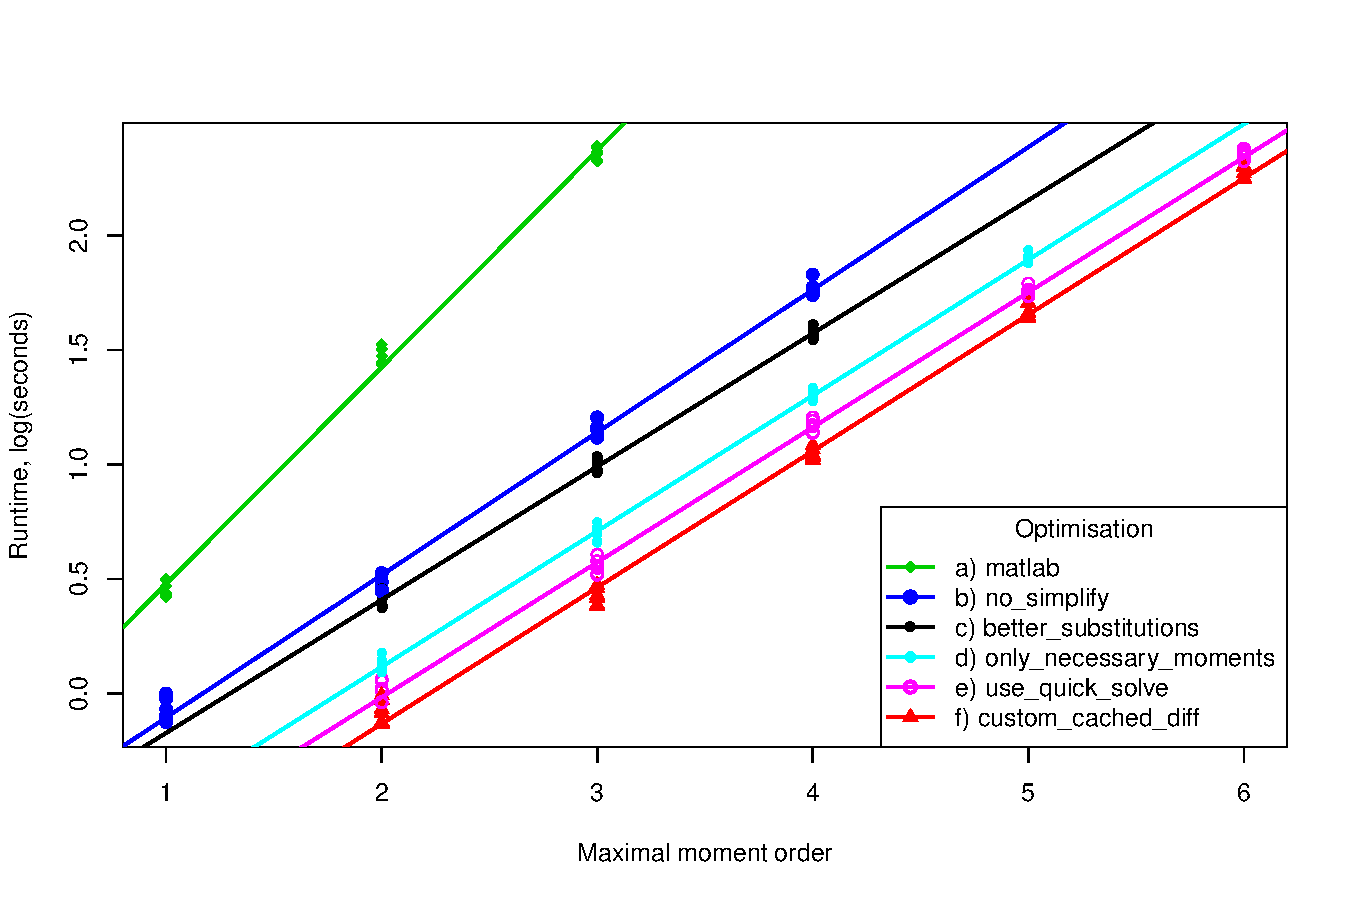
\includegraphics[width=0.95\textwidth{}]{../figure_mea_speed/mea_speed.pdf}
\caption{\emph{Cumulative performance improvement of symbolic 
calculations resulting from optimisation}.
The processing time for computing log-normal closure on \pft{} model with different \gls{maxord}s were measured for original Matlab implementation (a) and different optimisations (b$-$f).
In a first place, the calls to \texttt{sympy.simplify()} where removed (b). 
Then, \texttt{sympy.xreplace()} was used instead of \texttt{sympy.substitute()} (c). 
Generating an $(n-s) \times (n_2-s + 1)$ matrix (d), as opposed to an $(n-s) \times (n-s + 1)$ one, also increase speed.
Implementing a simplified equation solver instead of using \texttt{sympy.solve()} also resulted in a significant speed-up (e). 
Finally, caching (memorisation) \texttt{sympy.diff()} allowed even better performance.
The time complexity appears exponential ($O(2^n)$, where $n$ is the maximal moments order) in every case, 
%Interestingly, the slopes between, a ($0.95$) and c ($0.58$), and b ($0.62$) and c were significantly different ($p-value <10^{-15}$ and $p-value = 3 \times 10^{-4}$, respectively; t-test on the slopes of the linear regression). 
%No significant difference was found between the slopes of the subsequent optimisations (c$-$f). 
%However, the intercepts were significantly smaller between each consecutive optimisations after c) ($p-value < 10^{-6}$ for all; t-test on the intercepts of the linear regression).
Nine replicates were performed on the same CPU. 
For optimisation c$-$f, values corresponding to \gls{maxord} moments lower than two were removed because of the inherent inaccuracy in measuring very short durations.
}
\label{fig:mea_speed}
\end{figure}

\quentintodo{move the stats here}

Reorganising, profiling and rewriting the code resulted in incremental significant performance improvements of symbolic computations in \means{} compared to the original \mat{} code.
For instance, with the same \pft{} system and closure method, 
we predict that computation up to \gls{ode}s up $8^{th}$ order will take 46 minutes with \means{}, 5 hours after the first optimisation (fig.~\ref{fig:mea_speed}b) and as much as 148 days with the original implementation.
These improvement have allowed us to explore the performance of MEA in higher depth, and will hopefully contribute to make \gls{mea} realistically usable for systems with more species and reactions.

\subsubsection{Evaluating Expressions Efficiently}

As mentioned in the introduction to this section, the reduction of computational cost was the main reason for developing of approximation methods.
In order to be able to explore the approximation methods in more depth,
we needed to make the generation of the set of equations as efficient as possible, as mentioned in the previous section.

Generating a set of equations (\ie{} and \gls{ode} problem) is generally only the first step.
In most cases, the result is used to perform simulations with different parameters.
As a consequence, the same \gls{ode} problem will be generated once, and used many times.
Typically, a user would spend some time to generate an set of equation using \gls{mea}, and then use this \gls{ode} problem to perform hundreds of simulations.
Therefore, it was extremely important to assess and try to improve numerical evaluation performance.
 
%Even though it is a great improvement from the original prototype, 46 minutes is still a long time to wait for the computer to do the number crunching. 
%We can accept to wait this long, however, as we only need to do that once for a set of equations -- the next time we intend to do that, we can just read the previous set from a file.

%Evaluating these expressions is a completely different story however.
%Since we need to evaluate each expression hundreds, if not thousands of times when performing the simulations of the system,
% we want to make these tasks as efficient as possible, as every microsecond counts. 

In order to minimise the overhead of computations, we use the {\tt autowrap} module, built into {\tt sympy} to compile our numeric expressions into \texttt{C}
and then wrap the same \py{} interface around them so the end user does not see any difference.
This process bears some overhead, of course, as the system needs to be compiled for every simulation.

We notice that the expressions for a given set of equation could be compiled once and reused for all subsequent simulations on this set of equations.
Therefore, we used caching to keep precompiled expressions in memory.
 
As a consequence, the overhead is present only in the first evaluation of expressions, whilst all other evaluations are an order of magnitude faster.
This performance improvement is illustrated in the tutorial \autoref{sec:reuse_of_simulation_objects}.

\subsubsection{Comparing the Performance of Different \gls{ode} Solvers}

The symbolic expression evaluation speed, whilst incredibly important, contributes only partially to the scalability of the simulation procedures.
The performance of numerical \gls{ode} solvers themselves also plays a critical role.

These solvers differ by their respective options, heuristics or algorithms.
Choice of the \emph{best} solver for an \acrlongpl{ode} system depends very much on the particular problem to simulate.
However certain solvers tend to be more generally adopted than others\cite{andersson_workbench_2012}.

CVODE\cite{hindmarsh_sundials_2005} is an example of one of the most widely used solvers.
As described in \autoref{sec:ode_simulations}, we implement two variants of this solver, \verb#ode15s# and \verb#cvode#.
Both solvers point to the same back-end implementation of CVODE provided by \verb#assimulo# package\cite{andersson_christian_assimulo:_????}.
The only diference is that \verb#ode15s# solver's default parameters mimics the eponymous \mat{} solver.

In order to measure the runtime performance of the solvers, we performed a set of simulations of the \acrlong{mea} of the \pft{} model.
We deliberately chose two sets of parameters: one that we know is fairly stable and easy to simulate with, so called \emph{safe} parameter set,
and another parameter set that is known to cause the trajectories to become stiff and therefore cause problems to the solvers.
We call the latter parameter set the \emph{unsafe}.
 
\begin{figure}[tb]
   \centering
   \begin{subfigure}[t]{0.45\textwidth}
       \includegraphics[width=\textwidth]{../pipeline/task-output/solver-runtimes/runtimes-ode15s.pdf}
       \caption{\texttt{ode15s}}
       \label{fig:runtimes-safe-unsafe-ode15s}
   \end{subfigure}
   ~
   \begin{subfigure}[t]{0.45\textwidth}
       \includegraphics[width=\textwidth]{../pipeline/task-output/solver-runtimes/runtimes-euler.pdf}
       \caption{Euler}
       \label{fig:runtimes-safe-unsafe-euler}
   \end{subfigure}
   
    \caption{Comparison of the time taken for the {\tt ode15s} and Euler solvers to simulate a system, with respect to two parameter sets.
     The ``safe'' parameter set is very stable, while the ``unsafe'' one leads to stiff problems, which are harder to solve.
    The time axis is in log-scale. Regression lines through the marked points is represented.
    Note that the number of equations increases exponentially with maximum order, essentially making this a log-log plot.}
\label{fig:runtimes-safe-unsafe}
\end{figure}

\texttt{ode15s} solver was more performant for the safe parameter set (fig.~\ref{fig:runtimes-safe-unsafe-ode15s}).
Heuristic solvers tend to automatically adjust the step size depending on the problem in hand, adjusting for the rate of stochastic events being simulated.
It is therefore expected that they would perform worse for stiff problems, where the timeframes between the events become shorter and shorter, which requires more time steps.

In contrast, Euler solver, uses a constant step size, thus the runtimes for the two parameter sets are equal (\autoref{fig:runtimes-safe-unsafe-euler}).

Since \gls{ode} solvers are inherently heuristic, their CPU performance may suffer considerably for unstable systems.

Besides CVODE solvers, our package is able to perform simulations with seven other solvers, using completely different algorithms.
The complete list of available solvers used is available in the documentation\citationneeded{refer to docs}.
Naturally, we were then interested in assessing, in the same fashion, all nine available solvers for these two parameter sets (\autoref{fig:solver-runtimes}).
This exhaustive analysis reviled that \texttt{ode15s} was the most performant solver for this problem.
It outperformed other solvers for both safe and unsafe parameter sets.
Interestingly, \texttt{dopri5} appeared to scale better for unsafe parameter sets, and could be interesting when working with high \gls{maxord}s.
Surprisingly, \texttt{rodas}, which has been described as an very competitive solver for stiff \gls{ode}\cite{sandu_benchmarking_1997},
performed poorly on this case.

Using an appropriate solver can improve numerical performance by an order of magnitude (\autoref{fig:solver-runtimes}).
Therefore, we advise users to benchmark different solvers on their specific problems if numerical evaluation speed is critical (\ie{} for parameter inference).
In addition, advanced users can optimise the numerous options of each solvers in order improve performance.
Although we cannot conclude that \texttt{ode15s} is the fastest solver for all \gls{mea} problems,
it seems to be a reasonable default solver.

\begin{figure}[bt]
    \centering
    \includegraphics[width=\textwidth]{../pipeline/task-output/solver-runtimes/runtimes-all.pdf}
    \caption{\emph{Comparison of all solver runtimes.}
    The runtime of nine different solvers were compared for a safe (left side) and an unsafe (right side) parameter set.
    Regression lines through the marked points is represented in a different colour for each solver.
    Solvers are sorted, top to bottom, by increasing performance in the legend.
    \texttt{ode15s} was globally the fastest solver.
    }
    \label{fig:solver-runtimes}
\end{figure}


In order to improve performance, we have compared solvers on the basis of their speed.
However, they also differ in their accuracy and stability. 
In fact, most solvers trade-off accuracy and speed\cite{sandu_benchmarking_1997}.
This was investigated in  \sauliustodo{ref to new section once I create it}.

\subsection{Moment Expansion and Closure}

In \gls{mea} the time derivative of each central moment (moments of orders higher than one) is expressed in terms of higher order moments.
This behaviour has no upper bound and continues up to moments of infinite order.
Since we cannot evaluate these expressions in the limit analytically, it is necessary to ``close'' the expansion by providing a closed form for the higher order moments.
This also makes the method an ``approximation" rather than an exact method.

In the original work \cite{ale_general_2013}, higher order central moments are assumed to be equal to zero.
This is very convenient, but remains a strong and not necessarily valid assumption.

As an alternative, parametric probability distribution can be used to express moments of arbitrary orders.
For instance, a multivariate normal distribution is parametrised only by means (\ie{} first order raw moment)
and a covariance matrix (\ie{} second order central moments).
As a consequence, it is possible to express any arbitrary moment from means, variances and covariances.
A promising area of research involves closing moment expansion by parametric forms for highest order central moments (instead of assuming them to be null).
Preliminary work \cite{lakatos_preparation_2014} suggests that using a parametric distributions for \gls{mea} is, in some cases, a better approximation.
In addition, Ale \emph{et al.} predicted that ``including more moments would improve the estimation''\cite{ale_general_2013}.

The dramatic improvement in performance compared to the \mat{} prototype (see \autoref{sec:optimising_mea}) has rendered the exploration of higher-order and parametric moment closures possible.
Therefore, we were naturaly interested in investigating the effect of \gls{maxord} and different type of closures on the quality of the approximation.
Figure~\ref{fig:max_order_and_closure_on_distance_summary} summarises our results on the \pft{} model. 
The detail of generated trajectories for two representative \gls{maxord}s and one species are shown in
\autoref{fig:max_order_and_closure_on_distance_trajectories}.

\begin{figure}[t]
    \centering
    \includegraphics[width=0.95\textwidth]{../pipeline/task-output/FigureP53Summary/FigureP53Summary-pdf-7.pdf}
    \caption{\emph{Effect of different closure methods and \gls{maxord} on simulation accuracy}. The \pft{} system was modelled using \gls{mea} with five types of closure and for \gls{maxord} up to seven.
Resulting trajectories were all compared to an average of 5000 \gls{ssa} simulations using sum of square distance.
Distance is in log scale. Missing values indicate solver failure for that particular set of parameters.}
    \label{fig:max_order_and_closure_on_distance_summary}
\end{figure}

The \pft{} system, with parameters from \cite{ale_general_2013}, was investigated.
As mentioned above approximation accuracy is expected to increase with the \gls{maxord}, \ie{} distance to \gls{ssa} obtained should decreases
 as \gls{maxord} increases.
For normal and scalar closures, we observe this trend up to \gls{maxord} of six.
However, this does not stand for seventh order moment.

Normal distribution closure, with maximum order of seven, performed worse than the sixth order and fith order for the same closure (fig.~\autoref{fig:max_order_and_closure_on_distance_summary}).
We could not obtain the result for the seventh order closure using the standard scalar and univariate normal closure
because the ODE solver failed to simulate the problem.
This usually indicates a ``stiff'' \gls{ode} problem\citationneeded{stiff odes}.
In this case, the trajectories generated seem to `mismatch' the trajectory obtained from the \gls{ssa} simulations by
large a margin (fig.~\autoref{fig:max_order_and_closure_on_distance_trajectories}, right panel).
% (\emph{purple line, subplot on the right-hand-side}).

The reason for this behaviour is uncertain. It could either be a limitation of the approximation method, or a numerical limitation of the available \gls{ode} solver.
It is hard to know which explanation is more likely since we cannot test the two hypotheses separately.
Interestingly, we observed a similar behaviour with all of the solvers tested, which is further explored in \sauliustodo{link to my section where we study the phenomenon on larger scale with different solvers}.

Note that for even \gls{maxord}s, normal and scalar closure methods return identical result.
It means that when the \gls{maxord} is even,  the parametric expression of an odd (the next) order moment was used for closure.
Normal distribution is symmetrical. One consequence is that odd central moments are always zero.
For instance, the skewness (\ie{} third order central moment) of a normal distribution is zero.
Therefore, this behaviour is perfecty normal.


\begin{figure}
    \centering
    \includegraphics[width=0.95\textwidth]{../pipeline/task-output/FigureP53Simple/FigureP53Simple-pdf-7.pdf}
%~
    \caption{\emph{Complete trajectories of a single species (\pft) for max order three and seven are shown} 
    Black lines indicate the average of \gls{ssa} simulations. 
    Missing lines, compared to the legend in \autoref{fig:max_order_and_closure_on_distance_summary} indicate solver failure.}
    \label{fig:max_order_and_closure_on_distance_trajectories}
\end{figure}

 
For log-normal closure, the ground-truth trajectory seems to be well approximated when the \gls{maxord} is three.
However the approximation becomes less and less accurate for higher \gls{maxord} moments.
A deeper look at the trajectories indicate that, in this latter case,
oscillations are damped too quickly. (fig.~\autoref{fig:max_order_and_closure_on_distance_trajectories}, red lines, right panel).
This contrasts with normal closure, where the oscillation amplitude increases.

Interestingly, for even \gls{maxord} (\ie{} 2, 4, 6) log-normal closures generated \gls{ode}s which, despite our efforts, could not be numerically solved.

Finally, it seems that the results obtained from multivariate distribution closures and univariate distribution closures,
 which do not model the covariance terms, are the similar for this particular system.
This is not true for all of the systems.
For instance, we have observed that in the \emph{hes1}, it is advantageous to model covariance (data not show).
\quentintodo{put hes1 exple if time}

Surprisingly, higher order moment closure did not necessarily result in better approximations.
In addition, our results indicate that there might be a complex interaction between the type of closure and the \gls{maxord}.
Unfortunately, this makes it difficult to define \emph{a priori} which closure and \gls{maxord} should be used for a given system.
These unexpected results lead us explores this phenomenon on wider scale of parameters\sauliustodo{link to the section}.

\subsection{Choice of Parameters Affects \acrshort{mea} Accuracy}
\label{sec:hit-and-miss}

\todo[inline]{New Section: Please review. I particularly struggled with how to refer to the special points in the plot, anyone have any ideas?}

\begin{figure}
    \centering
    \foreach \order in {1,...,4}{
        \begin{subfigure}[t]{0.45\textwidth}
            \includegraphics[width=\textwidth]{{../pipeline/task-output/FigureHitAndMiss/FigureHitAndMiss-pdf-\order-scalar-True-0.0_40.0_0.1-ode15s--5000-0.1}.pdf}
            \caption{Max order $= \order$}
            \label{fig:hit-and-miss:ode15s:\order}
        \end{subfigure}
        ~
    }
    
    \foreach \order in {5,...,7}{
        \begin{subfigure}[t]{0.31\textwidth}
            \includegraphics[width=\textwidth]{{../pipeline/task-output/FigureHitAndMiss/FigureHitAndMiss-pdf-\order-scalar-True-0.0_40.0_0.1-ode15s--5000-0.1}.pdf}
            \caption{Max order $= \order$}
            \label{fig:hit-and-miss:ode15s:\order}
        \end{subfigure}
        ~
    }
    \caption{\emph{Contour plots of the sum-of-squares distance between the \gls{mea} approximated trajectory and the \gls{ssa} simulated trajectory for scalar closure and \texttt{ode15s} solver}.
    The grid of distances was calculated by sampling each of the two parameters $c_2$ and $c_4$ at $0.1$ intervals and comparing the simulated trajectories to the \gls{ssa} trajectory.
    Areas where \gls{ode} solver has failed are marked by black-and-white stripes.
    The four points indicated with $\bullet$, $\ast$, $\times$ and $\blacksquare$ represent sets of interests studied in other figures.
    The set of parameters used in \autoref{fig:max_order_and_closure_on_distance_summary} is indicated by a $\star$.
    Note that as the maximum order parameter increases, so does the relatively low-distance area.
    However, the area in which the system is stable shrinks at a similar rate.
    It also appears that even \gls{maxord}s are more stable than the odd ones.}
    
    \label{fig:hit-and-miss:ode15s}
\end{figure}

In the previous section, we address the difficulty to predict which maximum order to use in order to optain the best approximation of the true behaviour of the system \emph{a priori}.
In this section we explore this behaviour in a global scale.
We were interested in how the choice of parameters affect both the ability of the \gls{ode} solvers to generate the trajectories and
the quality of these trajectories.

In order to achieve this, we first fixed all the parameters of \pft{} model but $c_2$ and $c_4$ to the same values as in previous section.
The remaining two parameters were varied by $0.1$ increments of within the ranges $c_2 \in [1.5, 2.7)$ and $c_4 \in [0.6, 2.7)$ (where previously $c_2=1.7$ and $c_4=0.93$).
For ever every combination of these parameters, the average of \gls{ssa} $5000$ trajectories was generated as ground truth data.

We then used the simulation routines in the \means{} package in order to generate a similar collection of approximated trajectories for each of these parameter sets.
The parameter sets for which the solvers failed to produce a result were also recorded.
We then computed the sum-of-squares distances between each of the simulated trajectories and the \gls{ssa} average, for the same parameter set.
Results are summarised by sets of contour plots (see \autoref{fig:hit-and-miss:ode15s}) which we discuss bellow.

\begin{figure}
    \centering
    \foreach \order in {1,2,4,7}{
        \begin{subfigure}[b]{0.25\textwidth}
            \includegraphics[width=\textwidth]{{../pipeline/task-output/FigureSSAvMEATrajectory/FigureSSAvMEATrajectory-pdf-\order-scalar-True-p53-90.0_0.002_1.6_1.1_2.1_0.96_0.01-70.0_30.0_60.0-0.0_40.0_0.1-ode15s--5000}.pdf}
            \caption{Max order $= \order$}
            \label{fig:hit-and-miss:bullet:\order}
        \end{subfigure}
        \hspace{-15pt} % compress the whitespace in each figure
    }
   \caption{\emph{The trajectories simulated for the parameter set marked by $\bullet$ symbol in \autoref{fig:hit-and-miss:ode15s} stay relatively similar as higher order moments are incorporated to the approximation.} Only one of the three species in the model is shown. The distance measure in the bottom right corner shows the distance computed for only these species.
   Note how similar are the trajectories pictured, despite the increasing order of the moment expansion.
   The trajectories for max order parameter that were not shown, are similar
    to the trajectories 2, 4 and 7 displayed in this figure (subplots\ref{fig:hit-and-miss:bullet:2}, \ref{fig:hit-and-miss:bullet:4}, \ref{fig:hit-and-miss:bullet:7}).}
   \label{fig:hit-and-miss:bullet}
\end{figure}

The distance landscape was not uniform. For instance, distance to \gls{ssa} could range from $100$ to $10^9$ (\autoref{fig:hit-and-miss:ode15s:1}).
Some areas of the parameter space seem to be easier to approximate than others.
Interestingly, in these areas, even the first-order moments are sufficient to capture the overall behaviour of the system accurately.
\autoref{fig:hit-and-miss:bullet:1} plots the first-order trajectories associated with the one of the easy-to-approximate parameters (indicated by $\bullet$ in the contour point).
We observe the typical damped oscillatory behaviour of the \gls{ssa} trajectory,
which results from individual trajectories stochastically getting out-of-phase with each other\cite{ale_general_2013}.
This observation rules out the hypothesis that the system behaviour becomes somewhat different in this region of the parameter space. 
Because of this, we could guess there is something intrinsic to the approximation method, rather than to the system itself, that reduces the need to model the higher-order moments of the system for these parameters.\quentintodo{Any better now?} 
Interestingly, the approximated trajectories for these regions stay nearly the same regardless of the order of moments simulated, as seen in \autoref{fig:hit-and-miss:bullet}. 
This strengthens the implication that higher order moments play no role in approximating the behaviour for this system at the particular parameter set.

Conversely, we can also see regions of the parameter space where the approximation seems to perform poorly,
\ie{} the bottom-right corner of the \autoref{fig:hit-and-miss:ode15s:1}.
This already hard-to-approximate area seems to have mountains of even harder to approximate values, such as the one indicated by a $\times$ symbol.
The trajectories at this last parameter set, together with the trajectories for the parameter set marked with a $\blacksquare$, are shown in \autoref{fig:hit-and-miss-interesting-points:ode15s:1}.
We can see that the oscillations for the $\blacksquare$ parameters are increasing, and not reducing, in amplitude -- completely opposite to what we observe in the \gls{ssa} data.
The amplitude becomes so large that the trajectory takes negative values for the concentrations (which is obviously incorrect).
 
The simulated trajectory for the $\times$ symbol, on the other hand, just plummets into the large negative values and does not recover.
Despite the fact that the concentrations obtained are not realistic, the trajectories generated do not match the true behaviour of the system.
Therefore both of these trajectories are not acceptable approximations of the true dynamic.


\begin{figure}
    \begin{subfigure}[t]{0.45\textwidth}
        \includegraphics[scale=0.6]{{../pipeline/task-output/FigureSSAvMEATrajectory/FigureSSAvMEATrajectory-pdf-1-scalar-True-p53-90.0_0.002_2.4_1.1_0.7_0.96_0.01-70.0_30.0_60.0-0.0_40.0_0.1-ode15s--5000}.pdf}
        \caption{Parameters ($\blacksquare$)}
        \label{fig:hit-and-miss-interesting-points:ode15s:1:blacksquare}
    \end{subfigure}
    ~
    \begin{subfigure}[t]{0.45\textwidth}
        \includegraphics[scale=0.6]{{../pipeline/task-output/FigureSSAvMEATrajectory/FigureSSAvMEATrajectory-pdf-1-scalar-True-p53-90.0_0.002_2.5_1.1_1.8_0.96_0.01-70.0_30.0_60.0-0.0_40.0_0.1-ode15s--5000}.pdf}
        \caption{Parameters ($\times$)}
        \label{fig:hit-and-miss-interesting-points:ode15s:1:times}
    \end{subfigure}
    \caption{\emph{The \gls{mea} approximated and \gls{ssa} simulated trajectories for the indicator points in the \autoref{fig:hit-and-miss:ode15s:1}}.
    Only one of the three species in the model is shown. The distance measure in the bottom right corner shows the distance computed for only these species.
    Note the different $y$ axis scale for the plots.}
    \label{fig:hit-and-miss-interesting-points:ode15s:1}     
\end{figure}

When maximum moment expansion order is set to two (\autoref{fig:hit-and-miss:ode15s:2}), the high-distance area contour seems to be smaller.
As a consequence, the $\times$ and $\blacksquare$ parameters are in a lower-distance zone.
The resulting trajectories for these two parameter sets are shown in \autoref{fig:hit-and-miss-interesting-points:ode15s:2}.
The trajectory for the parameter set $\blacksquare$ is particularly interesting (\autoref{fig:hit-and-miss-interesting-points:ode15s:2:blacksquare}) as it seems to show the oscillations that increase,
and then decrease in amplitude.
The behaviour for the other parameter set shows damped oscillations.
However, damping is too slow to match the results from the stochastic simulations.

\begin{figure}
    \begin{subfigure}[t]{0.45\textwidth}
        \includegraphics[scale=0.6]{{../pipeline/task-output/FigureSSAvMEATrajectory/FigureSSAvMEATrajectory-pdf-2-scalar-True-p53-90.0_0.002_2.4_1.1_0.7_0.96_0.01-70.0_30.0_60.0-0.0_40.0_0.1-ode15s--5000}.pdf}
        \caption{Parameters indicated by $\blacksquare$}
        \label{fig:hit-and-miss-interesting-points:ode15s:2:blacksquare}
    \end{subfigure}
    ~
    \begin{subfigure}[t]{0.45\textwidth}
        \includegraphics[scale=0.6]{{../pipeline/task-output/FigureSSAvMEATrajectory/FigureSSAvMEATrajectory-pdf-2-scalar-True-p53-90.0_0.002_2.5_1.1_1.8_0.96_0.01-70.0_30.0_60.0-0.0_40.0_0.1-ode15s--5000}.pdf}
        \caption{Parameters ($\times$)}
        \label{fig:hit-and-miss-interesting-points:ode15s:2:bullet}
    \end{subfigure}
    \caption{\emph{The \gls{mea} approximated and \gls{ssa} simulated trajectories for the indicator points in the \autoref{fig:hit-and-miss:ode15s:2}}.
    Only one of the three model species is shown.
    The distance measure in the bottom left corner is only for the species in the plot.}
    \label{fig:hit-and-miss-interesting-points:ode15s:2}     
\end{figure}

For even higher order moment expansions, we can see the solvers starting to struggle. For instance, the solver (\texttt{ode15s}) fails to simulate trajectories for a parameter set ($\blacksquare$) when the moment expansion is performed up to three moments (\autoref{fig:hit-and-miss:ode15s:3}). Other \gls{ode} solvers also struggle to produce any trajectories trajectories in this case (data not shown)\sauliustodo{This is individual-report material -- let's make it a "supplementary figures" alternative}.

As seen in the \autoref{fig:hit-and-miss:ode15s}, solvers tend to perform a bit better when the moment expansion is closed at even numbers. We can hypothesise that this indicates some implicit pairing between odd and even moment orders. This pairing would makes the systems unstable when the higher order moments to be set set to zero are even (what happens when max order is odd). 

From figure  \autoref{fig:hit-and-miss:ode15s:4} we can see the that the parameter $\times$ gets into a lower distance tier in when the maximum order is set to 4. This point then proceeds to move back to the border between the two tiers when the maximum order is set to 6 (\autoref{fig:hit-and-miss:ode15s:6}). 
The approximations at the parameter set marked with an $\ast$ become better as the low-distance area grows, and the trend continues for all of the maximum order data we have, as illustrated by \autoref{fig:hit-and-miss:ast}.

\begin{figure}
    \centering
    \foreach \order in {1,3,5,7}{
        \begin{subfigure}[b]{0.25\textwidth}
            \includegraphics[width=\textwidth]{{../pipeline/task-output/FigureSSAvMEATrajectory/FigureSSAvMEATrajectory-pdf-\order-scalar-True-p53-90.0_0.002_2.0_1.1_1.8_0.96_0.01-70.0_30.0_60.0-0.0_40.0_0.1-ode15s--5000}.pdf}
            \caption{Max order $= \order$}
            \label{fig:hit-and-miss:ast:\order}
        \end{subfigure}
        \hspace{-15pt} % compress the whitespace in each figure
    }
   \caption{\emph{The trajectories simulated for the parameter set marked by $\ast$ symbol in \autoref{fig:hit-and-miss:ode15s} become progressively better as higher order moments are incorporated to the approximation.} Only one of the three species in the model is shown. The distance measure in the bottom right corner shows the distance computed for only these species.
   Note the decreasing amplitude of solver trajectories that comes closer to the \gls{ssa} solution as more moments are incorporated. 
   }
   \label{fig:hit-and-miss:ast}
\end{figure}

To summarise, the performance of the \gls{mea} approximation using scalar moment closure strongly depends on the parameters being approximated. 
Areas of the parameter space that are approximated really well regardless of the number of higher-order moments used exist.
So do the areas where moment-expansion approximation seems to do badly regardless of the number of moments used. 
In the parameter space in between the two areas, the approximation seems to become more and more accurate as higher order moments are incorporated, as we would expect. 
Numeric \gls{ode} solvers tend to be more stable when the highest-order moments present in the approximation are even. 
This lack of stability has an interesting side effect that is most pronounced at closure order 7 (\autoref{fig:hit-and-miss:ode15s:7}), where it seems that approximation of the true behaviour is either fairly good, or the trajectories cannot be generated by the numeric \glspl{ode} solvers.

\subsubsection{Effect of Log-Normal Closure}


\begin{figure}
    \centering
    \foreach \order in {2,...,7}{
        \begin{subfigure}[t]{0.45\textwidth}
            \includegraphics[width=\textwidth]{{../pipeline/task-output/FigureHitAndMiss/FigureHitAndMiss-pdf-\order-log-normal-True-0.0_40.0_0.1-ode15s--5000-0.1}.pdf}
            \caption{Max order $= \order$}
            \label{fig:hit-and-miss:ode15s:log-normal:\order}
        \end{subfigure}
        ~
    }
    \caption{\emph{Contour plots of the sum-of-squares distance between the \gls{mea} approximated trajectory and the \gls{ssa} simulated trajectory for log-normal closure and \texttt{ode15s} solver}.
    The contour landscape has been computed in exactly the same manner as in \autoref{fig:hit-and-miss:ode15s} and the data interpretation can be performed in the same fashion. 
    Note that the distance values are much lower than the ones observed for scalar closure in general, directly indicating the log-normal moment closure approach to be promising. Interestingly, the decrease in the distance between \gls{ssa} and the simulated trajectory comes with the price of the system being less stable in general. Contrary to the pattern observed for scalar closure (\autoref{fig:hit-and-miss:ode15s}), even order moment closures seem to be more stable in log-normal scenario.}
    
    \label{fig:hit-and-miss:ode15s:log-normal}
\end{figure}

When we repeated the same procedure for moment closures using log-normal distribution, we were able to observe global decrease in the distances between the trajectories (\autoref{fig:hit-and-miss:ode15s:log-normal}) which is a strong indicator of the potential of distribution closure methods. 

Unfortunately, this decrease in distances does not come without a price. As we can see from the same set of contour plots, the solvers are less stable compared to when the scalar moment closure is used (which was pictured in \autoref{fig:hit-and-miss:ode15s}). 
For instance, the \verb"ode15s" solver fails to produce a single working trajectory when the maximum order is set to 6. 

Similarly to the scalar closure, the stability seems to be different for even and odd closure orders. 
Rather surprisingly, this pattern is opposite between the two methods -- scalar closure is more stable when maximum expansion order is set to even numbers, whereas the log-normal closure tends to be more stable for the odd ones.

Due to this inherent instability of the log-normal closure, the paradoxical observation, where the approximation is reasonable, provided that it is computable, as seen in high-order scalar closures (\autoref{fig:hit-and-miss:ode15s:7}) is more pronounced for log-normal closure method and is observable even at low-order moments.

These results are consistent with the preliminary results of log-normal closure investigations\cite{lakatos_preparation_2014}\todo{Can I cite Eszter here?}, and further indicate the promise of this work.

In conclusion, quantitative claims about the performance of \gls{mea} for a single parameter set must be taken with a grain of salt, as such performance depends strongly on the region of the parameter space that is being approximated and cannot be generalised for the whole parameter space.
However, general patterns can be observed when a large parameter space is considered at once. For instance, we were able to observe that log-normal parameter closure does better than scalar closure for the parameter ranges investigated on average. 
Similarly, the average approximation accuracy increases as the \gls{maxord} increases, but this has a negative impact on the solver stability.
Finally, there seems to be some pairing between odd and even order moments, that causes scalar closures with odd \gls{maxord}s become very unstable. The same observation is valid for log-normal closure methods, yet for even \gls{maxord}s.

\subsection{Parameter Inference using \acrlong{mea}}
Parameter inference procedure aims to obtain the correct parameter values for the system by exploring the parameter space and comparing the simulation trajectories with the experimental data.

To study the performance of the parameter inference procedure using \acrlong{mea},
we generated $5000$ \acrfull{ssa} simulations of the \pft{} with a certain parameter set. 
We believe this number of \gls{ssa} simulations is sufficient to capture the behaviour of this simple system in full.
Then, we used the average as an observed dataset from which to infer parameters.
In this way, we know exactly the values for the true parameters for every inference procedure.

In order to determine the accuracy of inference, we used the \pft{} model expressed only in terms of the first order moments.
This approximation was bound to be very inaccurate for the particular system, as higher order moments are necessary to capture the damped oscillations present in the means of \gls{ssa} simulations\cite{ale_general_2013}.


%\begin{figure}parameter pairs are pictured
%\centering
%\includegraphics[width=0.9\textwidth]{{../pipeline/task-output/SevenDimensionalInferenceFigure/SevenDimensionalInferenceFigure-pdf-ode15s--sum_of_squares-5000}.pdf}
%\caption{\emph{Distance landscape based on inference using all the parameters in \pft{} model.}
%In the parameter inference procedure, all seven parameters were free and started from the correct values.
%The parameters are aligned both horizontally and vertically to display the distance landscape obtained by comparing inferred trajectories with \gls{ssa} trajectories.}
%\label{fig:7_dimensional_parameter_space}
%\end{figure}


We deliberately started the inference from the correct parameter values, expecting an immediate convergence (\ie{} no movement in the parameter space).
Surprisingly, when parameters were free, the inference procedure was able to find a set of parameters, but very different from the correct ones, for which observed and theoretical trajectories are extremely similar (see \autoref{fig:range-free-parameter-inference}).
This result was unexpected, because, as mentioned previously, higher order moments are believed to be necessary to capture the complex behaviour of the system.

\begin{figure}
    \centering
    \includegraphics[width=0.95\textwidth]{{../pipeline/task-output/FigureInferenceStartEndSSA/Range-free-parameter-inference}.pdf}
    \caption{\emph{Incorrectly inferred parameter values can generate trajectories matching the empirical data at \gls{maxord} of $1$.}
Each column represents one species in the \pft{} model. 
The starting trajectories (red) were generated based on the true parameter values, 
as the inference procedure started from the true values, 
while the optimal trajectories (blue) were generated based on the inferred parameters, where all seven parameters were free.
Averaged trajectories from $5000$ \gls{ssa} simulations ($\times$) were regarded as experimental data to compare with the starting and optimal trajectories.}
    \label{fig:range-free-parameter-inference}
\end{figure}


%\sisitodo[inline]{Why don't we compare the SSA trajectories with these parameters somewhere as well, if there is time?}

In order to gain some insight into these unexpected inference results, we first attempted to restrict ourselves to a two-dimensional space, which is easier to understand.
To do this, we limited our parameter inference procedure to have only a pair of free parameters at a time (all other parameters were fixed to their true values).
We performed this for all combinations of two parameters.

\begin{figure}[tb]
    \centering
    \begin{subfigure}[t]{0.45\textwidth}
    \includegraphics[width=\textwidth, height=0.35\textheight]{{../pipeline/task-output/FigureInferenceStartEndSSA/Paired-parameters-c2-c6-y0}.pdf}
    \label{fig:parameter_pair_c2_c6}
    \caption{Parameter pair $c_2$ and $c_6$}
    \end{subfigure}
    ~
    \begin{subfigure}[t]{0.45\textwidth}
    \includegraphics[width=\textwidth, height=0.35\textheight]{{../pipeline/task-output/FigureInferenceStartEndSSA/Paired-parameters-c0-c1-y0}.pdf}
    \label{fig:parameter_pair_c0_c1}
    \caption{Parameter pair $c_0$ and $c_1$}
    \end{subfigure}
    ~
    \caption{\emph{Two out of four parameter pairs that can produce a perfect match between inferred optimal trajectories and SSA trajectories for one species in \pft{} model.}
    Trajectories for one out of three species are shown here for clear demonstration.
    The distance from the SSA trajectory for each species is displayed in each subfigure.
    Trajectories are simulated using maximum order of 1.}
    \label{fig:parameter_pairs}
\end{figure}

Interestingly, we were able to observe the same behaviour for the parameter pairs $c_2$ and $c_6$, $c_0$ and $c_1$, $c_1$ and $c_6$, and, finally, $c_0$ and $c_6$ (first two parameter pairs are pictured in the \autoref{fig:parameter_pairs}).
We then chose the pair of parameters that allowed the inference procedure to converge to a trajectory with minimal distance to the stochastic average: $c_2$ and $c_6$.


\begin{figure}
    \centering
    \begin{subfigure}[t]{0.25\textwidth}
    \includegraphics[width=\textwidth,height=0.2\textheight]{{../pipeline/task-output/SampleMultidimensionInferenceFigure/SampleMultidimensionInferenceFigure-pdf-1-scalar-True-90.0_0.002_1.704_1.1_0.93_0.96_0.7822-ode15s--90.0_0.002_1.704_1.1_0.93_0.96_0.7822-sum_of_squares-5000}.pdf}
    \caption{Contour plot}
    \label{fig:inference_phenomenon:maxorder:1:landscape}
    \end{subfigure}
    ~
    \begin{subfigure}[t]{0.7\textwidth}
    \includegraphics[width=\textwidth,height=0.2\textheight]{{../pipeline/task-output/FigureInferenceStartEndSSA/FigureInferenceStartEndSSA-1-scalar-c2-1.7040-c6-0.7822}.pdf}
    \caption{Trajectories}
    \label{fig:inference_phenomenon:maxorder:1:trajectories}
    \end{subfigure}
    ~
    \begin{subfigure}[t]{0.25\textwidth}
    \includegraphics[width=\textwidth,height=0.2\textheight]{{../pipeline/task-output/SampleMultidimensionInferenceFigure/SampleMultidimensionInferenceFigure-pdf-2-scalar-True-90.0_0.002_1.704_1.1_0.93_0.96_0.7822-ode15s--90.0_0.002_1.704_1.1_0.93_0.96_0.7822-sum_of_squares-5000}.pdf}
    \caption{Contour plot}
    \label{fig:inference_phenomenon:maxorder:1:landscape}
    \end{subfigure}
    ~
    \begin{subfigure}[b]{0.7\textwidth}
    \includegraphics[width=\textwidth,height=0.2\textheight]{{../pipeline/task-output/FigureInferenceStartEndSSA/FigureInferenceStartEndSSA-2-scalar-c2-1.7040-c6-0.7822}.pdf}
    \caption{Trajectories}
    \label{fig:inference_phenomenon:maxorder:1:trajectories}
    \end{subfigure} 
    \caption{\emph{Contour plots of distance to \gls{ssa} trajectory and trajectories for parameter inference performed with lower order \gls{mea} using \pft{} model showing incorrect inference.}
    Among seven parameters, only the values for $c_2$ and $c_6$ are inferred. The starting values were obtained from previous inference using the true parameter values.
    All the contour plots and the trajectories start with the same parameter values for inference.
    Each row displays a contour plot and corresponding trajectories using different \gls{maxord} in \gls{mea}.
    Note that the scales in the contour plots using different \gls{maxord}s are different.
    In the contour plots, the warmer the colour, the more distant the inferred trajectories are from the \gls{ssa} trajectories, and the numbers indicate the distance between optimal trajectories obtained from inference and the \gls{ssa} trajectories.
    In the trajectory plots, the distance between the optimal and \gls{ssa} trajectories are indicated at the bottom. 
    Although the optimal trajectories (blue) match with the \gls{ssa} trajectories ($\times$), the corresponding contour plot shows wrong values are inferred.
    The white space in the contour plots represent the unexplored parameter space.}
    \label{fig:inference_phenomenon:lower_order}
\end{figure}


Through further investigations in the contour plots and trajectories with different \gls{maxord}s, 
we found that inference based on lower order 
(see \autoref{fig:inference_phenomenon:lower_order}) 
\gls{mea} is more problematic than inference based on higher order \gls{mea} 
(see \autoref{fig:inference_phenomenon:higher_order}). 
This might because inference using lower order \gls{mea} approximations allows the \pft{} model to explore a region large enough that a low-distance area can be identified.
Yet the low-distance area  implies that the parameters values are easier to approximate with, but not necessarily the true parameter values.
For example, optimal trajectories simulated at lower order can mabut not necessarily the true parameter valuestch with the \gls{ssa} trajectories completely, which is also consistent with the result in \autoref{sec:hit-and-miss}. 
Moreover, in \autoref{fig:inference_phenomenon:maxorder:1:landscape}, 
the starting point of parameter inference, \ie{} true values, is labelled as a high-distance zone. 
This unexpected high-distance can be explained by \gls{mea} unable to capture the damped oscillatory behaviour of the system for this set of parameters without higher order moments, as illustrated by the starting trajectories in \autoref{fig:inference_phenomenon:maxorder:1:trajectories}. 
 
%What is surprising to observe, however, is that the landscape is not relatively level \ie{} the approximation is not equally bad for all parameter sets. There is a clear pool of parameters, where no high-order information is needed to approximate this oscillatory behaviour.

Generally, inference based on higher order \gls{mea} is able to produce more realistic results, as reflected by less distance between the starting trajectories and the \gls{ssa} trajectories, and shallower distance gradients in the contour plots (see \autoref{fig:inference_phenomenon:higher_order}). The slightly more correct inference may be a result of more accurate \gls{mea} approximation. However, the parameter inference process is still not stationary and is able to drift away from the correct set of parameters.


\begin{figure}
    \centering
    \begin{subfigure}[b]{0.25\textwidth}
    \includegraphics[width=\textwidth,height=0.2\textheight]{{../pipeline/task-output/SampleMultidimensionInferenceFigure/SampleMultidimensionInferenceFigure-pdf-3-scalar-True-90.0_0.002_1.704_1.1_0.93_0.96_0.7822-ode15s--90.0_0.002_1.704_1.1_0.93_0.96_0.7822-sum_of_squares-5000}.pdf}
    \end{subfigure}
    ~
    \begin{subfigure}[b]{0.7\textwidth}
    \includegraphics[width=\textwidth,height=0.2\textheight]{{../pipeline/task-output/FigureInferenceStartEndSSA/FigureInferenceStartEndSSA-3-scalar-c2-1.7040-c6-0.7822}.pdf}
    \end{subfigure}   
     ~  
    \begin{subfigure}[b]{0.25\textwidth}
    \includegraphics[width=\textwidth,height=0.2\textheight]{{../pipeline/task-output/SampleMultidimensionInferenceFigure/SampleMultidimensionInferenceFigure-pdf-4-scalar-True-90.0_0.002_1.704_1.1_0.93_0.96_0.7822-ode15s--90.0_0.002_1.704_1.1_0.93_0.96_0.7822-sum_of_squares-5000}.pdf}
    \end{subfigure}
    ~
    \begin{subfigure}[b]{0.7\textwidth}
    \includegraphics[width=\textwidth,height=0.2\textheight]{{../pipeline/task-output/FigureInferenceStartEndSSA/FigureInferenceStartEndSSA-4-scalar-c2-1.7040-c6-0.7822}.pdf}
    \end{subfigure}   
   
    \begin{subfigure}[b]{0.25\textwidth}
    \includegraphics[width=\textwidth,height=0.2\textheight]{{../pipeline/task-output/SampleMultidimensionInferenceFigure/SampleMultidimensionInferenceFigure-pdf-5-scalar-True-90.0_0.002_1.704_1.1_0.93_0.96_0.7822-ode15s--90.0_0.002_1.704_1.1_0.93_0.96_0.7822-sum_of_squares-5000}.pdf}
    \end{subfigure}
    ~
    \begin{subfigure}[b]{0.7\textwidth}
    \includegraphics[width=\textwidth,height=0.2\textheight]{{../pipeline/task-output/FigureInferenceStartEndSSA/FigureInferenceStartEndSSA-5-scalar-c2-1.7040-c6-0.7822}.pdf}
    \end{subfigure}
    
    \begin{subfigure}[b]{0.25\textwidth}
    \includegraphics[width=\textwidth,height=0.2\textheight]{{../pipeline/task-output/SampleMultidimensionInferenceFigure/SampleMultidimensionInferenceFigure-pdf-6-scalar-True-90.0_0.002_1.704_1.1_0.93_0.96_0.7822-ode15s--90.0_0.002_1.704_1.1_0.93_0.96_0.7822-sum_of_squares-5000}.pdf}
    \end{subfigure}
    ~
    \begin{subfigure}[b]{0.7\textwidth}
    \includegraphics[width=\textwidth,height=0.2\textheight]{{../pipeline/task-output/FigureInferenceStartEndSSA/FigureInferenceStartEndSSA-6-scalar-c2-1.7040-c6-0.7822}.pdf}
    \end{subfigure}
   
\caption{\emph{Contour plots of distance to \gls{ssa} trajectory and trajectories for parameter inference performed with higher order \gls{mea} using \pft{} model.}  
    Among seven parameters, only the values for $c_2$ and $c_6$ were inferred. The starting values were obtained from previous inference using the true parameter values.
    All the contour plots and the trajectories start with the same parameter values for inference.
    Each row displays a contour plot and correspondent trajectories using different \gls{maxord} in \gls{mea}.
    Note that the scale in the contour plots at different orders can be different.
    In the contour plots, the warmer the colour, the more distant the inferred trajectories are from \gls{ssa} trajectories, and the numbers indicate the distance between optimal trajectories and \gls{ssa} trajectories.
    The white space in the contour plots represent the parameter space not explored by the system. 
    In the trajectory plots, the distance between the optimal (blue) and \gls{ssa} trajectories ($\times$) are indicated at the bottom.}
\label{fig:inference_phenomenon:higher_order}
\end{figure}


%\sisitodo[inline]{Fix the big figure so you can refer to individual parts from text}

In conclusion, recovering the correct parameter set remains challenging, even with higher order \gls{mea} approximations. This observation raises concerns about the validity of parameter inference approaches using \gls{mea} approximation. 
